\section{\large 先行研究}
\par Vissersらによって,電気泳動による正負荷電コロイド粒子混合系のレーン形成現象についての研究が行われている\cite{Teun}.
Visserらは,レーン形成現象を実験とシミュレーションの両方を用いて解析している.Fig. \ref{preworksnap}は実験とシミュレーション両方でのスナップショットである.
(b,c)は実験での結果,(d,e)はシミュレーションの結果をそれぞれ表している.
(b,d)では外部電場$\boldsymbol{E}=30\,\textrm{kV/m}$,(c,e)では$\boldsymbol{E}=110\,\textrm{kV/m}$の電場がかかっている.
外部電場が大きくなると,よりはっきりとレーンが形成されていることが確認できる.
ここで,赤が正に帯電した粒子,緑が負に帯電した粒子をそれぞれ表している.
\begin{figure}[H]
\centering
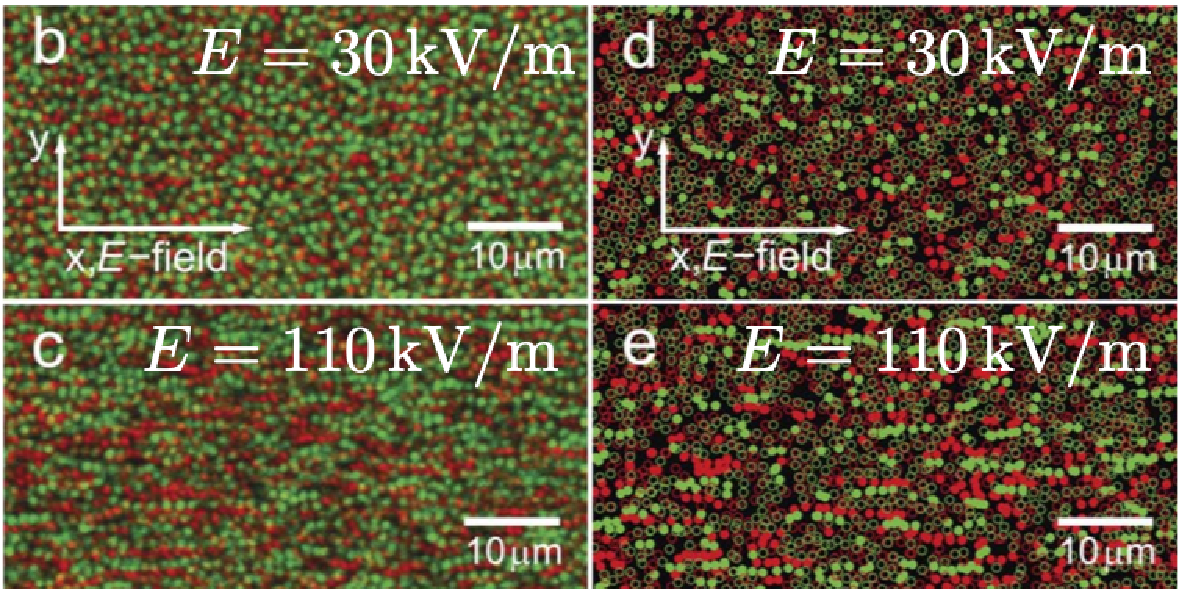
\includegraphics[scale = 0.7]{figures/prework.pdf}
\caption{レーン形成の様子}
\label{preworksnap}
\end{figure}
\noindent
また,先行研究ではレーン形成率$\Phi$が導入されており,レーン形成が定量的に評価されている.
さらに,シミュレーションでは,外部電場が大きくなればなるほど,レーンがより強く形成されることが報告されている.

先行研究では流体力学的相互作用を無視したシミュレーションが行われているが,レーン形成のような動的な挙動においては,流体は重要な役割を果たすことが知られている.
そこで,本研究では流体力学的相互作用を考慮したレーン形成現象の解析を行った.
